\section{Désigner un référentiel (3 points)}
\begin{questions}
	
\question[3] Dans quel référentiel, parmi ceux proposés ci-dessous, a personne sur le tapis roulant en fonctionnement est-elle immobile ?
 
\end{questions}

\begin{multicols}{2}
	 
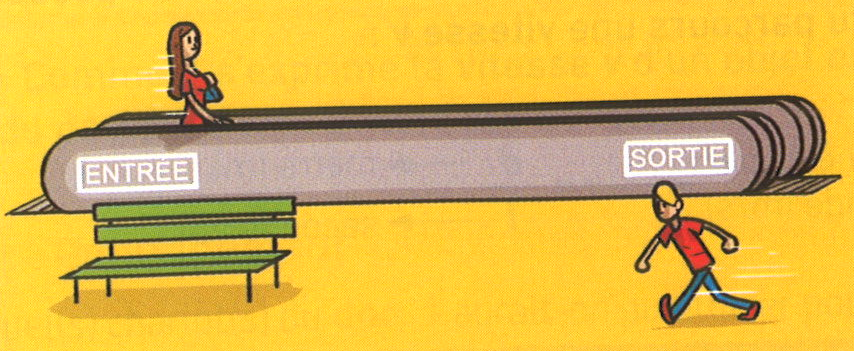
\includegraphics[scale=0.3]{tapis}
 
 \begin{enumerate}
 	\item Le tapis roulant.
 	\item La personne qui marche à l'extérieur du tapis roulant.
 	\item La banc. 
 \end{enumerate}



\end{multicols}
\fillwithdottedlines{3.5cm}